\documentclass[11pt, fleqn]{article}

\usepackage[usenames,dvipsnames,svgnames,table]{xcolor}
\usepackage{amsmath}
\usepackage{amsfonts}
\usepackage[margin=1in]{geometry} % To set the margin widths
\usepackage{graphicx}
\usepackage{listings}
\usepackage{multirow}
\usepackage{tabularx}
\usepackage{varioref}
\usepackage[noabbrev,capitalize]{cleveref}
\usepackage[group-separator={,}]{siunitx}
\usepackage{subcaption}
\usepackage{titlesec}
\usepackage{lscape}
\usepackage{bm}
\usepackage{chngpage}
\usepackage[titletoc,toc,title]{appendix}

\renewcommand\thesection{\arabic{section}}
\renewcommand\thesubsection{\thesection\alph{subsection}}

\lstset{
  frame=single,
  basicstyle=\ttfamily,% print whole listing small
  language=R,
  aboveskip=3mm,
  belowskip=3mm,
  showstringspaces=false,
  columns=flexible,
  numbers=none,
  commentstyle=\color{ForestGreen},
  stringstyle=\color{Maroon},
  breaklines=true,
  breakatwhitespace=true,
  tabsize=2,
  literate={<-}{{$\gets$}}1 {~}{{$\sim$}}1
}

\sisetup{output-exponent-marker=\textsc{e}}

\setlength{\parskip}{12pt} % Sets a blank line in between paragraphs
\setlength\parindent{0pt} % Sets the indent for each paragraph to zero

\begin{document}

\title{Homework \#4\\
Digital and Algorithmic Marketing (37304-01)}
\author{
Brian Chingono, Will Clark, Matthew DeLio, Jonathan Stevens (\textbf{Group \#8})\\
University of Chicago Booth School of Business}

\maketitle

\section{Message Combinations} % Question 1

The number of possible message combinations that can be tested, or full factorial, is 1,024 message combinations. This number of combinations is a result of the number of factors that are being tested (7), and the number of levels for each factor.  The levels for the factors, in order from 1 to 7 are 4,4,2,2,2,4 and 2.  Thus, the number of combinations is equal to the product $4\times4\times2\times2\times2\times4\times2 = 1,024$.    

\section{Logit Model Estimation} % Question 2

We estimate two logistic regression models, one for an open rate and one for a click rate:
\[ \log{\frac{p}{1-p}} = \bm{X}^{\prime} \bm{\beta} + \bm{\varepsilon} \]
where $p$ is the probability of a click or an open, $\bm{X}$ is the model matrix containing indicator variables for each factor/level combination, and $\bm{\beta}$ is the vector of estimated coefficients. We report the coefficients for the click and open models in \cref{tab:logit_results}, as well as the odds multipliers for each coefficient (which are just $\exp{\beta_j}$).
% latex table generated in R 3.2.5 by xtable 1.8-0 package
% Tue May  3 21:07:17 2016
\begin{table}[ht]
\centering
\caption{Logistic Regression Coefficients} 
\label{tab:logit_results}
\begin{tabular}{rrrrr}
  \hline
 & $\beta_j^{\text{open}}$ & $\exp(\beta_j^{\text{open}})$ & $\beta_j^{\text{click}}$ & $\exp(\beta_j^{\text{click}})$ \\ 
  \hline
\textsf{intro:L2} & 0.0127 & 1.01 & 0.00146 &    1 \\ 
  \textsf{intro:L3} & 0.0177 & 1.02 & 0.122 & 1.13 \\ 
  \textsf{intro:L4} & 0.00882 & 1.01 & -0.00526 & 0.995 \\ 
  \textsf{headline:L2} & 0.0106 & 1.01 & 0.0987 &  1.1 \\ 
  \textsf{headline:L3} & 0.00577 & 1.01 & 0.0802 & 1.08 \\ 
  \textsf{headline:L4} & 0.00837 & 1.01 & 0.0456 & 1.05 \\ 
  \textsf{main\_text:L2} & -0.00898 & 0.991 & -0.0116 & 0.989 \\ 
  \textsf{button:L2} & 0.000971 &    1 & -0.0101 & 0.99 \\ 
  \textsf{action:L2} & -0.0194 & 0.981 & 0.136 & 1.15 \\ 
  \textsf{purpose:L2} & 0.00639 & 1.01 & -0.0222 & 0.978 \\ 
  \textsf{purpose:L3} & -0.00481 & 0.995 & -0.0973 & 0.907 \\ 
  \textsf{purpose:L4} & -0.000423 &    1 & -0.0938 & 0.911 \\ 
  \textsf{symbol:L2} & 0.015 & 1.02 & -0.00475 & 0.995 \\ 
   \hline
\end{tabular}
\end{table}

We can make a few observations:
\begin{itemize}
\item The effects in the click model are all stronger than the effects in the open model. Put differently, message optimization has a much stronger effect on click behavior than it does on open behavior. The odds multipliers on the open model are all very close to 1; the odds multipliers on the click model vary from 0.907 to 1.13.
\item Far and away, the two most important elements of a message for generating clicks are to use \textsf{action L2} and \textsf{intro L3}. They increase the odds of a click by 12.6 and 12.9 percent, respectively.
\item Conversely, a bad \textsf{purpose} will really drag down a message's click rate. The pair of \textsf{purpose L3} and \textsf{purpose L4} decrease the odds of a click by 9.2 percent and 8.9 percent, respectively.
\end{itemize}

\section{Prediction} % Question 3

We generated a full factorial of all 1,024 message combinations. Using this full factorial, we used our models to estimate open probabilities and click probabilities for each of the 1,024 message combinations. For comparison purposes, we also calculated the open and click probabilities for the control sample.

Our results are in \cref{fig:q3_hist} below. As shown in those histograms, there is a significant difference between the baseline click and open probabilities of the control message versus the estimated probabilities from our full factorial. Even the worst message in the test set is better than the baseline message.

\begin{figure}[!htb]
  \centering
  \caption{Histogram of Predicted Probabilities vs. Control}
  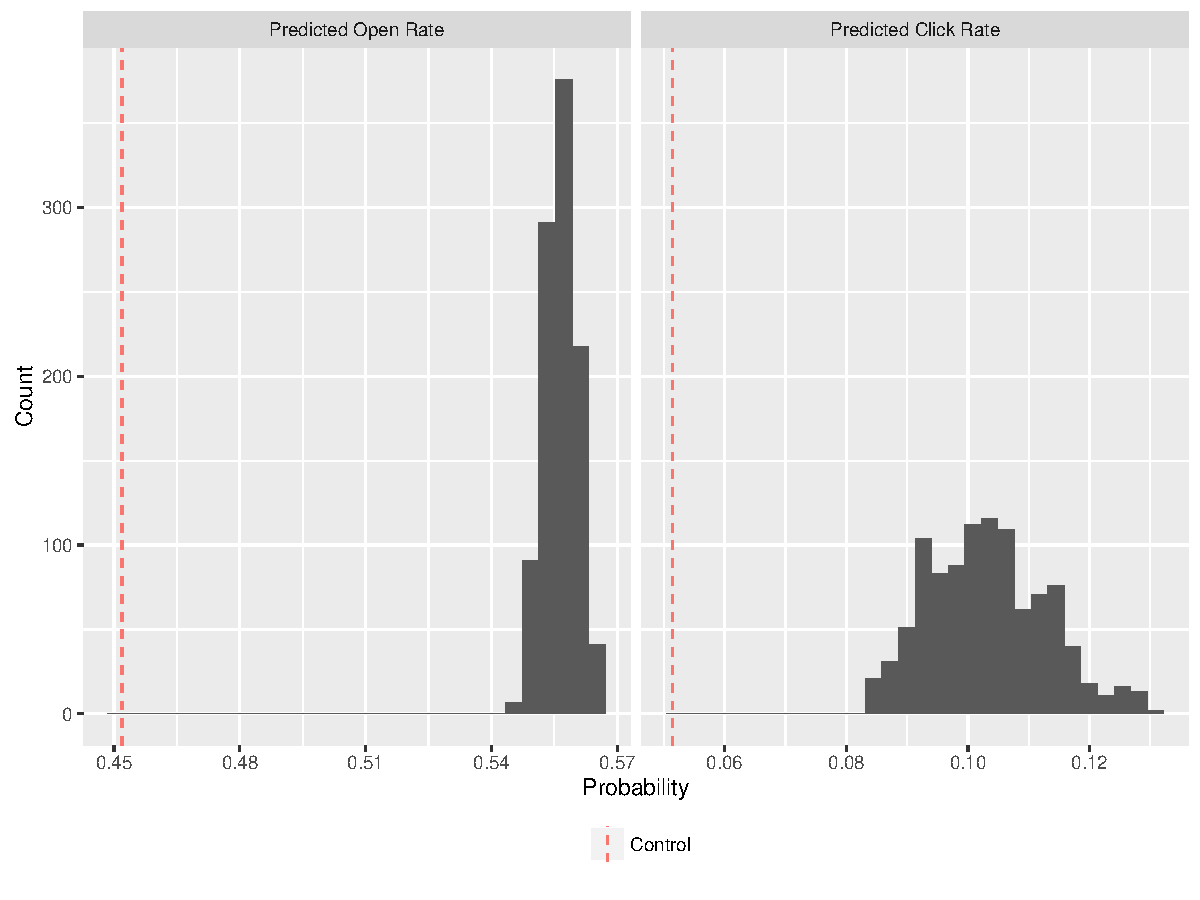
\includegraphics[scale=0.5]{q3_hist.pdf}
  \label{fig:q3_hist}
\end{figure}

In terms of optimal message combinations, the best combination for the fitted open probability is outlined in \cref{tab:best_open}. This message had a predicted open rate of 56.7 percent and a predicted click rate of 11.2 percent (placing it in the 79th percentile of emails ranked by click rate).

The optimal combination for the fitted click probability  is listed in \cref{tab:best_click}. This message had a predicted open rate of 55.6 percent (placing it in the 47th percentile of emails ranked by open rate) and a predicted click rate of 13.0 percent.

% latex table generated in R 3.2.5 by xtable 1.8-0 package
% Tue May  3 20:58:47 2016
\begin{table}[ht]
\centering
\caption{Features of Best Open Rate Message} 
\label{tab:best_open}
\begin{tabular}{rll}
  \hline
 & Level & Description \\ 
  \hline
intro & L3 & MORE Everything has been activated \\ 
  headline & L2 & CONGRATS! \\ 
  main\_text & L1 & Make the most of your new plan’s savings \& shareable data... \\ 
  button & L2 & Symbol Before text \\ 
  purpose & L2 & Have a Look \\ 
  symbol & L2 & >> \\ 
   \hline
\end{tabular}
\end{table}

% latex table generated in R 3.2.5 by xtable 1.8-0 package
% Tue May  3 20:57:17 2016
\begin{table}[ht]
\centering
\caption{Features of Best Click Rate Message} 
\label{tab:best_click}
\begin{tabular}{rll}
  \hline
 & Level & Description \\ 
  \hline
intro & L3 & MORE Everything has been activated \\ 
  headline & L2 & CONGRATS! \\ 
  main\_text & L1 & Make the most of your new plan’s savings \& shareable data - add a new device today! \\ 
  button & L1 & Symbol after text \\ 
  purpose & L1 & Take a Look \\ 
  symbol & L1 & ▶ \\ 
   \hline
\end{tabular}
\end{table}


These two messages are generally similar because they both have an introduction of \textit{``MORE Everything has been activated''} and they both have a headline of \textit{``CONGRATS!''}. Moreover, the main text in both of these messages is \textit{``Make the most of your new plan’s savings \& shareable data - add a new device today!''}. These similarities may be the parts of the message that pique the readers' interest. The differences between the messages are in terms of the button positioning, the call to action, the purpose, and the symbol.

\end{document}

% \input{.tex}

% \begin{figure}[!htb]
%   \centering
%   \caption{}
%   \begin{subfigure}[b]{0.49\textwidth}
%     \caption{}
%     \includegraphics[width=\textwidth]{.pdf}
%     \label{fig:}
%   \end{subfigure}
%   \hfill
%   \begin{subfigure}[b]{0.49\textwidth}
%     \caption{}
%     \includegraphics[width=\textwidth]{.pdf}
%     \label{fig:}
%   \end{subfigure}
% \end{figure}

% \begin{figure}[!htb]
%   \centering
%   \caption{}
%   \includegraphics[scale=.5]{.pdf}
%   \label{fig:}
% \end{figure}